\documentclass{article}
\usepackage[T1]{fontenc}
\usepackage{amsmath, amssymb, amsthm}
\usepackage[margin=1in]{geometry}
\usepackage{hyperref}
\usepackage{tikz}
\usetikzlibrary{arrows.meta}

\newtheorem{theorem}{Theorem}
\newtheorem{proposition}[theorem]{Proposition}
\newtheorem{corollary}[theorem]{Corollary}
\theoremstyle{definition}
\newtheorem{definition}[theorem]{Definition}
\newtheorem{example}[theorem]{Example}
\theoremstyle{remark}
\newtheorem{remark}[theorem]{Remark}
\newtheorem*{problem*}{Open Problem}

\title{\textbf{\Large Contexts and pseudocontexts}}

\author{\textbf{Mirko Navara$^1$ and Karl Svozil$^2$}\\[.5em]
$^1$ Faculty of Electrical Engineering,\\
Czech Technical University in Prague, Czechia\\[.5em]
$^2$ Institute for Theoretical Physics,
TU Wien, Austria
}

\date{}

\begin{document}
\maketitle

\begin{abstract}
In the projection lattice of a finite-dimensional Hilbert space, an orthogonal basis -- a \emph{context} -- is characterised by the property that its atomic probabilities sum to one on every state. We study a weakening of this condition, in which two tuples of atoms induce the same probability sum on every state. Such pairs are called \emph{pseudocontexts}. In finite dimension this is equivalent to two distinct rank-one decompositions of the same positive operator, placing the notion naturally among finite frame-theoretic constructions. Size $k=1$ is trivial; size $k=2$ already admits genuinely nonorthogonal examples; and, in fact, examples exist for every $k\ge 2$. We present the operator formulation, give a general explicit construction, illustrate the symmetric $k=3$ case with a figure, and list the remaining classification problems.
\end{abstract}

\section{Introduction}

Let $L$ be the lattice of projections in a Hilbert space of finite dimension $n\ge 3$.
Its atoms (minimal non-zero elements) correspond to one-dimensional subspaces, represented by nonzero vectors.
States are described by probability measures $P\colon L\to[0,1]$.
We denote by $S(L)$ the set of all states on $L$.

Vectors $a_1,\ldots,a_n$ form a \emph{context} if they compose an orthogonal basis.
In this case (and only in this case), they satisfy
\begin{equation}
\forall P\in S(L): \sum_{i=1}^n P(a_i)=1\,.
\label{eq:context}
\end{equation}

The present note concerns weaker additive identifications obtained by comparing two tuples of atoms that are not required to be orthogonal. Such \emph{pseudocontexts} are quantum-logical shadows of orthomodular-lattice constructions of Mayet--Navara--Rogalewicz~\cite{MayetNR} and have direct physical meaning: they encode state-independent empirical equivalences between families of generally noncommuting observables. The answer is simple: pseudocontexts already exist for $k=2$, and, more generally, for every $k\ge 2$.

\section{Preliminaries}

Throughout, $H$ is a complex Hilbert space with $\dim H=n\ge 3$, and $L=L(H)$ is the orthomodular lattice of its closed subspaces.
Its atoms correspond to one-dimensional subspaces, or equivalently to \emph{rays} spanned by nonzero vectors.
We identify an atom with any representative unit vector $a$ and write $P_a=|a\rangle\langle a|$ for the orthogonal projection onto the ray it spans.

A \emph{state} is a map $P\colon L\to[0,1]$ with $P(I)=1$ that is finitely additive on orthogonal families.
By Gleason's theorem~\cite{Gleason}, every state arises from a density operator $\rho$ via
\begin{equation}
P(a)=\operatorname{tr}(\rho\,P_a), \qquad \rho\ge 0,\ \operatorname{tr}\rho=1.
\label{eq:gleason}
\end{equation}
The key consequence we use repeatedly is that two self-adjoint operators that agree on every state are equal as operators.

\section{Contexts and pseudocontexts}

The operator form of \eqref{eq:context} is elementary and is the starting point for everything that follows.

\begin{proposition}[Contexts]\label{prop:context}
Unit vectors $a_1,\dots,a_n\in H$ form an orthonormal basis if and only if
\begin{equation}
\sum_{i=1}^{n} P_{a_i}=I.
\label{eq:context-op}
\end{equation}
\end{proposition}

\begin{proof}
The forward implication is immediate.
For the converse, fix $j$ and evaluate \eqref{eq:context-op} on the vector $a_j$:
\[
1=\langle a_j, I a_j\rangle
=\sum_{i=1}^{n} |\langle a_i,a_j\rangle|^2.
\]
The term with $i=j$ already contributes $1$, so all others must vanish.
Hence $\langle a_i,a_j\rangle=0$ for $i\neq j$.
As this holds for every $j$, the family is orthonormal, and being of size $n$ in an $n$-dimensional space it is an orthonormal basis.
\end{proof}

Combined with \eqref{eq:gleason}, Proposition~\ref{prop:context} recovers \eqref{eq:context} as a state-theoretic characterisation of orthogonal bases.

\begin{definition}[Pseudocontext]\label{def:pc}
Let $k\ge 1$. A \emph{pseudocontext of size $k$} is a pair of $k$-tuples of atoms $(a_1,\dots,a_k)$, $(b_1,\dots,b_k)$ such that the underlying set $\{a_1,\dots,a_k,b_1,\dots,b_k\}$ has cardinality $2k$ and
\begin{equation}
\forall P\in S(L):\quad \sum_{i=1}^{k} P(a_i)=\sum_{i=1}^{k} P(b_i).
\label{eq:pc}
\end{equation}
\end{definition}

A pseudocontext is called \emph{genuine} if neither $k$-tuple is a context.

By \eqref{eq:gleason}, condition \eqref{eq:pc} is equivalent to the operator identity
\begin{equation}
T \;:=\; \sum_{i=1}^{k} P_{a_i}
\;=\;
\sum_{i=1}^{k} P_{b_i},
\label{eq:opid}
\end{equation}
which we call the \emph{structure operator} of the pseudocontext.
Thus pseudocontexts are precisely pairs of distinct rank-one decompositions of a single positive operator.
This places them naturally among finite frame-theoretic constructions: contexts are the special case in which the structure operator is the identity on the relevant subspace; in general, pseudocontexts are rank-one decompositions of a common positive operator.
If the common operator is proportional to the identity on its support, the family is a tight frame; after normalisation on that support, one obtains a POVM.

\section{The smallest cases}

\begin{proposition}[Size $k=1$]\label{prop:k1}
There is no pseudocontext of size $k=1$.
\end{proposition}

\begin{proof}
The condition $P(a_1)=P(b_1)$ for all $P\in S(L)$ is equivalent, via \eqref{eq:gleason}, to $P_{a_1}=P_{b_1}$.
This rank-one identity forces $a_1$ and $b_1$ to span the same ray, contradicting distinctness.
\end{proof}

\begin{corollary}[Size $k=2$]\label{cor:k2}
There are genuinely nonorthogonal pseudocontexts of size $k=2$.
\end{corollary}

\begin{proof}
Embed $\mathbb C^2$ into $\mathbb C^n$ as the span of the first two basis vectors and set
\[
u_\pm=\left(\frac{\sqrt3}{2},\,\pm\frac12,\,0,\ldots,0\right),\qquad
v_\pm=\left(\frac{\sqrt3}{2},\,\pm\frac{i}{2},\,0,\ldots,0\right).
\]
Then
\[
P_{u_+}+P_{u_-}
=
P_{v_+}+P_{v_-}
=
\begin{pmatrix}
3/2 & 0\\
0 & 1/2
\end{pmatrix}\oplus 0_{n-2}.
\]
The four rays are distinct, and within each pair the vectors are nonorthogonal.
\end{proof}

\begin{remark}[Real vs.\ Complex for $k=2$]
It is worth noting that genuinely nonorthogonal pseudocontexts of size $k=2$ strictly require complex Hilbert spaces. In a real Hilbert space, the requirement that a trace-2 positive operator $A$ admits a rank-one decomposition $A = P_c + P_d$ algebraically rigidly fixes the rays up to sign, forcing the two sets of rays to be identical. The availability of a continuous complex phase is what unlocks the $k=2$ pseudocontexts in Corollary~\ref{cor:k2}. For $k \ge 3$, however, pseudocontexts can be constructed entirely over the reals, as demonstrated in Section~6.
\end{remark}

\section{Pseudocontexts of every size $k\ge 2$}

\begin{theorem}[Complex-phase construction]\label{thm:allk}
Let $H$ contain an orthonormal pair $e_1,e_2$.
Fix an integer $k\ge 2$, let $\omega=e^{2\pi i/k}$, choose $\alpha\in(0,\pi/2)$, and choose $\phi\in\mathbb R$ such that $e^{i\phi}$ is not a $k$th root of unity.
Define unit vectors
\[
a_j=\cos\alpha\,e_1+\sin\alpha\,\omega^j e_2,\qquad
b_j=\cos\alpha\,e_1+\sin\alpha\,e^{i\phi}\omega^j e_2,
\qquad j=0,\dots,k-1.
\]
Then the $2k$ rays spanned by the $a_j$ and $b_j$ are pairwise distinct, and
\[
\sum_{j=0}^{k-1} P_{a_j}
=
\sum_{j=0}^{k-1} P_{b_j}
=
k\bigl(\cos^2\alpha\,P_{e_1}+\sin^2\alpha\,P_{e_2}\bigr).
\]
Hence $(a_0,\dots,a_{k-1})$ and $(b_0,\dots,b_{k-1})$ form a pseudocontext of size $k$.

If $\alpha\neq\pi/4$, then the pseudocontext is genuine.
\end{theorem}

\begin{proof}
Write $c=\cos\alpha$ and $s=\sin\alpha$.
For each $j$ we have
\[
P_{a_j}
=
c^2 P_{e_1}+s^2 P_{e_2}
+cs\bigl(\omega^{-j}|e_1\rangle\langle e_2|+\omega^{j}|e_2\rangle\langle e_1|\bigr),
\]
and
\[
P_{b_j}
=
c^2 P_{e_1}+s^2 P_{e_2}
+cs\bigl(e^{-i\phi}\omega^{-j}|e_1\rangle\langle e_2|
+e^{i\phi}\omega^{j}|e_2\rangle\langle e_1|\bigr).
\]
Summing over $j=0,\dots,k-1$ and using
\[
\sum_{j=0}^{k-1}\omega^j=0
\]
gives
\[
\sum_{j=0}^{k-1}P_{a_j}
=
\sum_{j=0}^{k-1}P_{b_j}
=
k\bigl(c^2P_{e_1}+s^2P_{e_2}\bigr).
\]

For distinctness, suppose $a_j=\lambda a_\ell$.
Since $c\neq 0$, comparing the first coordinates gives $\lambda=1$, and then $\omega^j=\omega^\ell$, so $j=\ell$.
Similarly, if $a_j=\lambda b_\ell$, then $\lambda=1$ and hence $\omega^j=e^{i\phi}\omega^\ell$, which is impossible by the choice of $\phi$.
The same argument shows that the $b_j$ are pairwise distinct rays.

Finally,
\[
\langle a_j,a_\ell\rangle = c^2+s^2\omega^{\ell-j}.
\]
This can vanish only if $c^2=s^2$ and $\omega^{\ell-j}=-1$, so if $\alpha\neq\pi/4$ then no two distinct rays in the same $k$-tuple are orthogonal.
The same holds for the $b_j$.
Hence the pseudocontext is genuine.
\end{proof}

\begin{remark}
At the special value $\alpha=\pi/4$, the structure operator becomes
\[
\frac{k}{2}\,I_{\operatorname{span}\{e_1,e_2\}},
\]
so the construction yields a unit-norm tight frame on the two-dimensional support.
For $k=2$ this is just a context; for $k\ge 3$ it gives a highly symmetric pseudocontext.
\end{remark}

\section{A symmetric $k=3$ example}

Surprisingly, the case $k=3$ has a very transparent planar representation.
It is the finite-dimensional analogue of the Mercedes--Benz frame.

\begin{example}[Mercedes--Benz type pseudocontext]\label{ex:mb}
Fix a two-dimensional subspace $V\subset H$ with orthonormal basis $(e_1,e_2)$, and fix an angle
\[
\theta\in(0,\pi)\setminus\{\pi/3,2\pi/3\}.
\]
Put, for $j=0,1,2$,
\[
a_j=\cos\Bigl(\tfrac{2\pi j}{3}\Bigr)e_1+\sin\Bigl(\tfrac{2\pi j}{3}\Bigr)e_2,
\qquad
b_j=\cos\Bigl(\tfrac{2\pi j}{3}+\theta\Bigr)e_1+\sin\Bigl(\tfrac{2\pi j}{3}+\theta\Bigr)e_2.
\]
Then the six rays are pairwise distinct, and
\[
\sum_{j=0}^{2}P_{a_j}
=
\sum_{j=0}^{2}P_{b_j}
=
\tfrac32\,I_V.
\]
Thus $\{a_0,a_1,a_2\}$ and $\{b_0,b_1,b_2\}$ form a pseudocontext of size $k=3$.
\end{example}

\begin{proof}
In the basis $(e_1,e_2)$, each projector has the form
\[
P_{\cos\varphi\,e_1+\sin\varphi\,e_2}
=
\begin{pmatrix}
\cos^2\varphi & \cos\varphi\,\sin\varphi\\
\cos\varphi\,\sin\varphi & \sin^2\varphi
\end{pmatrix}.
\]
For $\varphi_j=2\pi j/3$ and for $\varphi_j=\theta+2\pi j/3$, the trigonometric identities
\[
\sum_{j=0}^{2}\cos(2\varphi_j)=0,\qquad
\sum_{j=0}^{2}\sin(2\varphi_j)=0
\]
imply that the off-diagonal terms cancel, while the diagonal terms each sum to $3/2$.
Hence both sums equal $\frac32 I_V$.
The exclusion $\theta\notin \{\pi/3,2\pi/3\}$ guarantees that the two triples are distinct as sets of rays.
\end{proof}

\begin{figure}[ht]
\centering
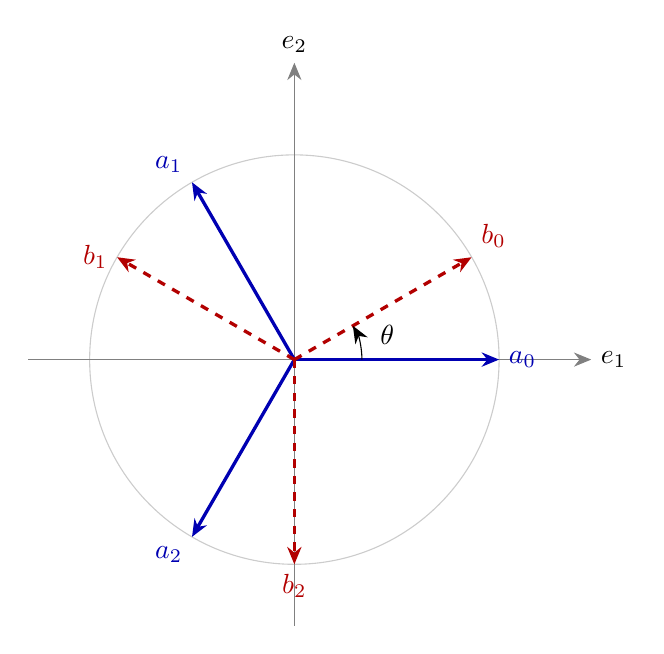
\begin{tikzpicture}[scale=2.6, >={Stealth[length=2.2mm,width=1.8mm]}]
  % reference circle
  \draw[thin, gray!40] (0,0) circle (1);
  % axes
  \draw[->, gray] (-1.3,0) -- (1.45,0) node[black, right] {$e_1$};
  \draw[->, gray] (0,-1.3) -- (0,1.45) node[black, above] {$e_2$};
  % a-vectors (solid, blue)
  \foreach \ang/\lbl/\pos in {%
      0/{a_0}/{right},%
    120/{a_1}/{above left},%
    240/{a_2}/{below left}}%
  {
    \draw[blue!70!black, very thick, ->] (0,0) -- (\ang:1);
    \node[blue!70!black, \pos] at (\ang:1) {$\lbl$};
  }
  % b-vectors (dashed, red), rotated by theta = 30 degrees
  \foreach \ang/\lbl/\pos in {%
     30/{b_0}/{above right},%
    150/{b_1}/{left},%
    270/{b_2}/{below}}%
  {
    \draw[red!70!black, very thick, dashed, ->] (0,0) -- (\ang:1);
    \node[red!70!black, \pos] at (\ang:1) {$\lbl$};
  }
  % rotation angle theta
  \draw[thin, ->] (0.33,0) arc (0:30:0.33);
  \node at (15:0.47) {$\theta$};
\end{tikzpicture}
\caption{The Mercedes--Benz pseudocontext of Example~\ref{ex:mb}, drawn for $\theta=\pi/6$. The solid blue rays $a_0,a_1,a_2$ and the dashed red rays $b_0,b_1,b_2$ are distinct unordered triples in the plane $V$, yet the associated rank-one projectors have the same sum $\tfrac32 I_V$.}
\label{fig:mb}
\end{figure}

\begin{remark}[Complex trine description]\label{rem:trine}
Example~\ref{ex:mb} has a compact complex analogue.
Let $\omega=e^{2\pi i/3}$ and embed $V$ into $\mathbb C^n$ as $\operatorname{span}\{e_1,e_2\}$.
The \emph{trines}
\[
u_j=\tfrac{1}{\sqrt2}\bigl(1,\omega^j,0,\ldots,0\bigr),
\qquad
v_j=\tfrac{1}{\sqrt2}\bigl(1,e^{i\phi}\omega^j,0,\ldots,0\bigr),
\qquad j=0,1,2,
\]
yield the same phenomenon after a change of basis in $V$.
The identity $1+\omega+\omega^2=0$ makes the off-diagonal entries of $\sum_j P_{u_j}$ cancel, giving the common structure operator $\tfrac32 I_V$.
This is the form most natural in frame-theoretic discussions and in connection with the Weyl--Heisenberg group.
\end{remark}

\begin{remark}[Nondegenerate structure operators]
The trine family is highly symmetric: its structure operator is a scalar multiple of the identity on its support.
More complicated examples with nondegenerate structure operators occur already in dimension three; see, for instance, the coordinatizations discussed in~\cite{NSvozil:pseudocontext,NSvozil:Escher}.
Such examples are useful when one wants to move beyond purely symmetric frame orbits.
\end{remark}

Similar constructions~\cite{MayetNR} were known when $L$ was a more general orthomodular lattice~\cite{Kalmbach}.
Some of these lattices can be represented as subsets of a Hilbert lattice~\cite{NSvozil:pseudocontext,NSvozil:Escher}.

\section{Physical interpretation and constraints}

A pseudocontext $(\{a_i\},\{b_i\})$ implements an empirical equivalence between two families of rank-one observables $A_i=P_{a_i}$ and $B_i=P_{b_i}$.
Although the operators within each family are generally noncommuting, the two linear functionals
\[
\rho \longmapsto \sum_i \operatorname{tr}(\rho A_i), \qquad
\rho \longmapsto \sum_i \operatorname{tr}(\rho B_i)
\]
agree on the whole state space.
Because the structure operators are identical, this equivalence is strictly state-independent.

In the language of quantum information theory, the collections $\{A_i\}$ and $\{B_i\}$ are distinct rank-one operator decompositions of the same positive operator.
If the common operator is proportional to the identity on its support, they form a tight frame; after normalisation on that support, one obtains a POVM.
From a foundational standpoint, this is a state-independent additive equivalence closely related to, but distinct from, Kochen--Specker-type contextuality~\cite{KochenSpecker,Cabello}.

\section{Open problems}

Having established the existence of pseudocontexts for every size $k\ge 2$ and isolated a simple $k=3$ illustration, we highlight the remaining questions regarding their deeper classification:

\begin{problem*}[Classification]
Classify, up to unitary equivalence, all pseudocontexts of size $k$ in $\mathbb C^n$.
Even for small $(k,n)$, the orbit structure is not yet transparent.
\end{problem*}

\begin{problem*}[Lattice representability]
Characterise which orthomodular lattices carrying a pseudocontext-type additive identification admit a faithful embedding into some $L(\mathbb C^n)$, sharpening the partial results of~\cite{NSvozil:pseudocontext,NSvozil:Escher}.
\end{problem*}

\begin{problem*}[Frame-symmetry characterisation]
Can one characterise pseudocontexts purely in terms of symmetries of the underlying rank-one frame --- for example, in terms of unitaries commuting with the structure operator and permuting the atoms of the two decompositions?
\end{problem*}

\section*{Acknowledgement}
This research was funded in part by the Austrian Science Fund (FWF) 10.55776/\allowbreak PIN5424624 and the Czech Science Foundation (GACR) 25-20013L.

\begin{thebibliography}{9}
 \bibitem{Gleason} Gleason, A.M.: Measures on the closed subspaces
 of a Hilbert space. \textit{J. Math. Mech.} \textbf{6} (1957), 885--893.

 \bibitem{Kalmbach} Kalmbach, G.: \textit{Orthomodular Lattices}.
 Academic Press, London, 1983.

 \bibitem{MayetNR} Mayet, R., Navara, M., Rogalewicz, V.:
 Orthomodular lattices with rich state spaces.
 \textit{Algebra Universalis} \textbf{43} (2000), 1--30.

 \bibitem{NSvozil:pseudocontext} Navara, M., Svozil, K.:
 Form of contextuality predicting probabilistic equivalence between two sets of three mutually noncommuting observables.
 \textit{Physical Review A} \textbf{109} (2024), 022222.
 DOI 10.1103/PhysRevA.109.022222

 \bibitem{NSvozil:Escher} Navara, M., Svozil, K.:
 Exploring Quantum contextuality with the quantum M\"obius--Escher--Penrose hypergraph.
 \textit{Physical Review A} \textbf{111} (2025), 042209.
 DOI 10.1103/PhysRevA.111.042209

 \bibitem{KochenSpecker} Kochen, S., Specker, E.P.:
 The problem of hidden variables in quantum mechanics.
 \textit{J. Math. Mech.} \textbf{17} (1967), 59--87.

 \bibitem{Cabello} Cabello, A., Estebaranz, J.M., Garc\'{\i}a-Alcaine, G.:
 Bell--Kochen--Specker theorem: A proof with 18 vectors.
 \textit{Phys. Lett. A} \textbf{212} (1996), 183--187.
\end{thebibliography}

\end{document}
